\begin{frame}
	\sectionpage
\end{frame}

\subsection{Présentation}
	\begin{frame}{Présentation}
		\begin{itemize}[<+->]
			\item Service web
			\item Basé sur Git
			\item Développé en Ruby on Rails \& Erlang
		\end{itemize}
	\end{frame}

\subsection{Fonctionnalités}
	\begin{frame}{Fonctionnalités}
	  \only<1>{
	    \begin{figure}
	      \centering
	      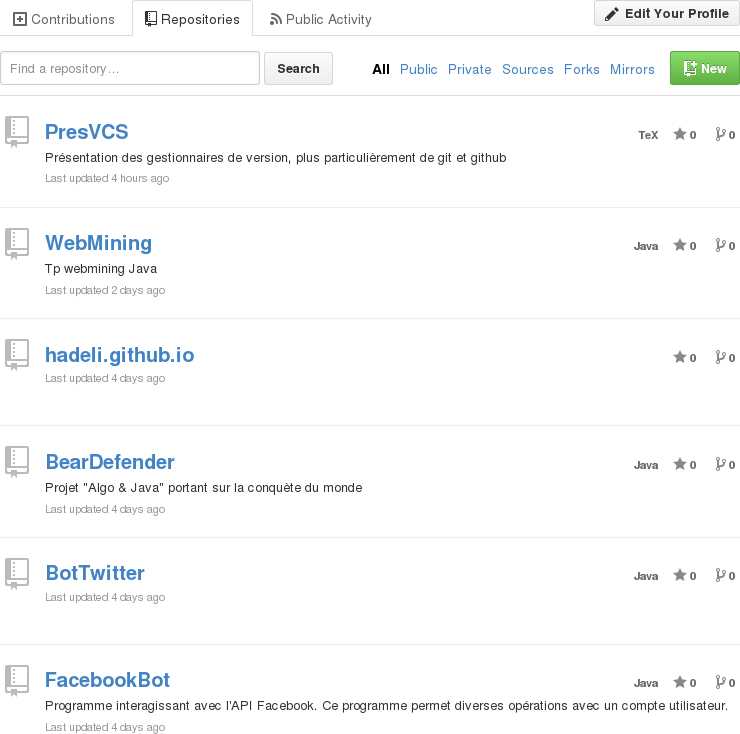
\includegraphics[width=60mm]{./Img/Repos.png}
	      % Repos.png: 0x0 pixel, 0dpi, 0.00x0.00 cm, bb=
	      \caption{Hébergements de projets}
	    \end{figure}
	  }
	\only<2>
	{
	  \begin{figure}
	    \centering
	    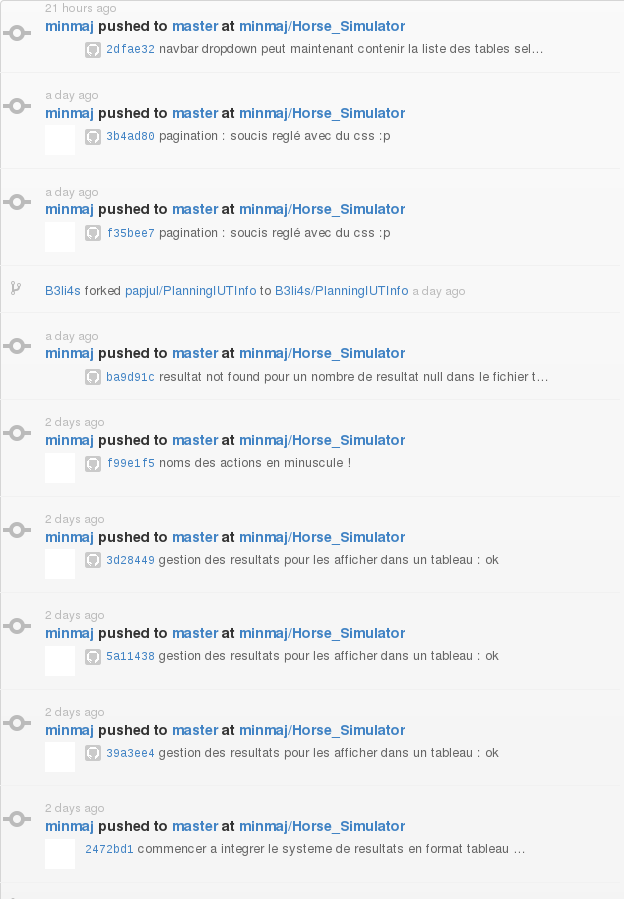
\includegraphics[width=45mm]{./Img/Social.png}
	    % Social.png: 0x0 pixel, 0dpi, nanxnan cm, bb=
	    \caption{Suivi de personnes et de projets}
	  \end{figure}

	}

	\only<3>
	{
	  \begin{figure}
	    \centering
	    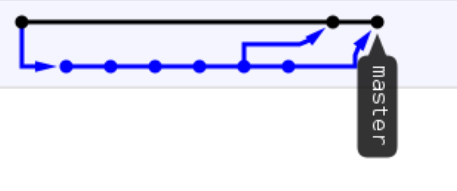
\includegraphics[width=85mm]{./Img/GraphRes.png}
	    % GraphRes.png: 0x0 pixel, 0dpi, nanxnan cm, bb=
	    \caption{Graphes de réseau}
	  \end{figure}

	}
	
	\only<4>
	{
	  \begin{figure}
	    \centering
	    \includegraphics[width=85mm]{./Img/Gists.png}
	    % Gists.png: 0x0 pixel, 0dpi, 0.00x0.00 cm, bb=
	    \caption{Système de pastebin}
	  \end{figure}
	}
	
	\only<5>
	{
	\begin{figure}
	  \centering
	  \includegraphics[width=95mm]{./Img/PagesPerso.png}
	  % PagesPerso.png: 0x0 pixel, 0dpi, 0.00x0.00 cm, bb=
	  \caption{Pages perso et Wiki disponible pour chaque dépot}
	 \end{figure}
	}

	\end{frame}

\subsection{Les outils}

  \begin{frame}{Windows}
  
    \begin{block}{En ligne de commande}
    \only<1,2>{
      \begin{itemize}
	\item<1>{\href{http://msysgit.github.io/}{\textit{\textcolor{blue}{Git for Windows}}}}
	\item<2>{\href{http://code.google.com/p/tortoisegit/}{\textit{\textcolor{blue}{Tortoise Git}}}}
      \end{itemize}
    }
    \end{block}
    
    \begin{block}{Avec interface graphique} 
      \only<3,4,5>{
      \href{http://windows.github.com/}{\textit{\textcolor{blue}{Github for Windows}}}
	\begin{itemize}
	  \item<3>{Facile d'acc\`es}
	  \item<4>{Possibilit\'e d'\'ecrire de longs messages de commit}
	  \item<5>{Affichage des diffs de mani\`ere ergonomique}
	\end{itemize}
      }
    \end{block}
    
  \end{frame}
  
  \begin{frame}{Linux}
  
    \begin{block}{En ligne de commande}
    \only<1>
    {
      \href{http://git-scm.com/book/fr/}{\textit{\textcolor{blue}{Documentation Git}}}
    }
    \end{block}
      
    \begin{block}{Avec interface graphique} 
    \only<2,3,4,5>
    {
      \begin{itemize}
	\item<2>{\href{http://git-cola.github.io/}{\textit{\textcolor{blue}{Git-cola}}}} 	\item<3>{\href{https://wiki.gnome.org/action/show/Apps/Gitg?action=show&redirect=Gitg}{\textit{\textcolor{blue}{Gitg}}}}
	\item<4>{\href{http://www.syntevo.com/smartgithg/}{\textit{\textcolor{blue}{SmartGit}}}}
	\item<5>{\href{http://www.collab.net/giteyeapp}{\textit{\textcolor{blue}{Git Eye}}}} 
      \end{itemize}
    }
    \end{block}
    
  \end{frame}
  
  \begin{frame}{IDEs}
  
    La majorit\'es des IDEs du march\'e ont une int\'egration de plusieurs VCS dont Git
    
    \only<2>
    {
      \begin{exampleblock}{Exemples :}
	\begin{itemize}
	\item PhpStorm, IntelliJ
	\item NetBeans
	\item Eclipse
	\end{itemize}
      \end{exampleblock}
    }
  \end{frame}
  
  \begin{frame}{Pour approfondir ...}
  
	  \begin{block}{Pour les commandes Git}
		  \href{http://try.github.io/}{\textit{\textcolor{blue}{Try Git}}}
	  \end{block}
	  
	  \begin{block}{TP à faire}
		  \href{http://bit.ly/iut-3}{\textit{\textcolor{blue}{TP Git}}}
	  \end{block}
	  
	  \begin{block}{Mon Github}
	    \href{http://github.com/hadeli}{\textit{\textcolor{blue}{Profil Github}}}\\
	    \href{http://hadeli.github.io}{\textit{\textcolor{blue}{Page Perso Github}}}
	  \end{block}
	  
  \end{frame}
